\section{Dynamic-MSV-Bench and Methodology}
\label{sec:benchmark}

We propose the \textbf{Dynamic-MSV-Bench}, which categorizes multi-shot prompts into two extreme stress-test scenarios to expose the "Double-Kill" dilemma of current models.

\begin{figure*}[ht]
    \centering
    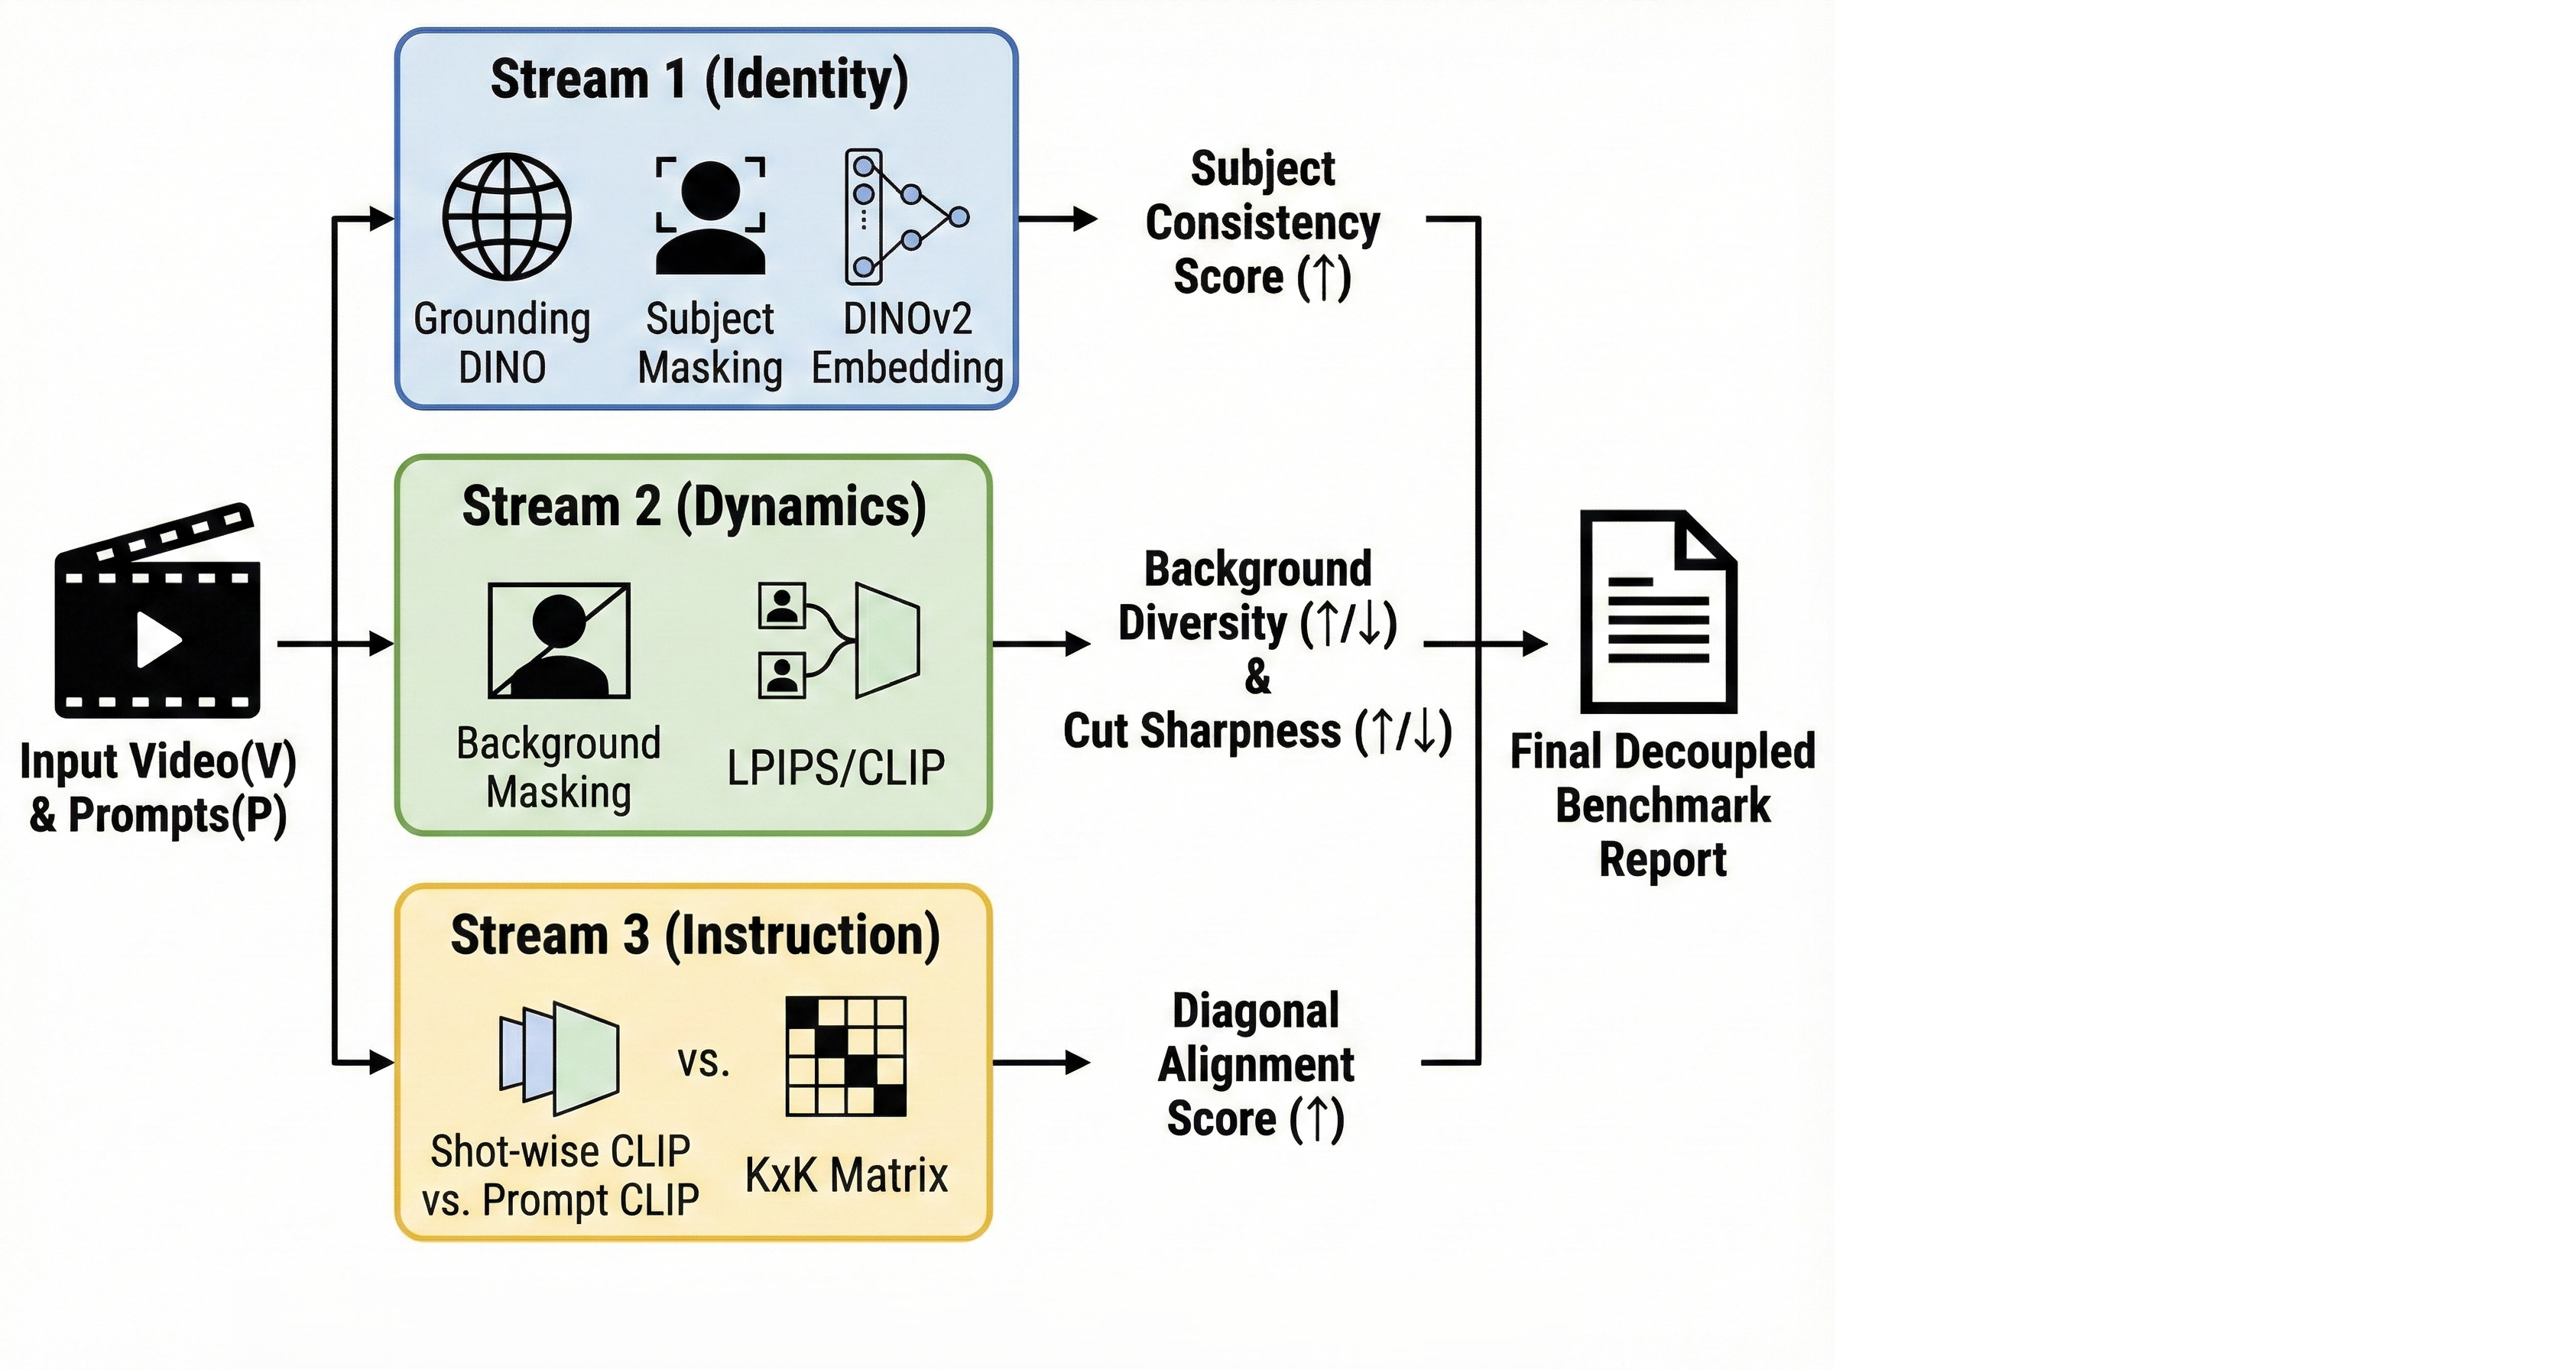
\includegraphics[width=\textwidth]{figures/fig2.jpg}
    \caption{Overview of our Decoupled 4D Evaluation Framework. Unlike holistic metrics like FVD, we process the input video through three independent streams to measure Subject Identity, Background Dynamics/Continuity, and Instruction Following (Diagonal Alignment) separately.}
    \label{fig:framework}
\end{figure*}

\begin{figure*}[ht]
    \centering
    \includegraphics[width=\textwidth]{figures/fig_AB.jpg}
    \caption{Conceptual comparison of our two evaluation tracks. (Left) \textbf{Track S: Semantic Leap} tests narrative diversity, requiring radical environment changes while preserving the subject. This track demands high Background Diversity and sharp cinematic cuts. (Right) \textbf{Track M: Motion Continuity} evaluates spatial integrity, where the background must remain consistent while the camera executes specific motions (Panning, Zooming, Tracking). Set M rewards low diversity and smooth spatial continuity.}
    \label{fig:sets_comparison}
\end{figure*}

\subsection{Track S: Semantic Leap (Narrative Diversity)}
Track S evaluates the model's ability to maintain a consistent subject while drastically shifting the semantic environment. 
The \textbf{Golden Rule for Track S} is defined as HIGH Background Diversity ($\uparrow$), HIGH Cut Sharpness ($\uparrow$), and HIGH Subject Consistency ($\uparrow$). 
\begin{itemize}
    \item \textbf{Background Diversity ($\uparrow$):} Since the narrative requires a leap between disparate locations (e.g., from a dense forest to outer space), the model must exhibit high variance in its environmental rendering. A low score here directly exposes the \textit{Static Trap}.
    \item \textbf{Cut Sharpness ($\uparrow$):} These environmental jumps should be depicted as distinct cinematic cuts. High sharpness at the shot boundaries ensures that the scenes are rendered independently, without "morphing" artifacts.
    \item \textbf{Subject Consistency ($\uparrow$):} Despite the radical background changes, the identity of the main protagonist must remain strictly preserved to maintain narrative logic across the leap.
\end{itemize}

\subsection{Track M: Motion Continuity (Spatial Integrity)}
Track M tests physical instructions while keeping the background stable. 
The \textbf{Golden Rule for Track M} is defined as LOW Background Diversity ($\downarrow$), LOW Cut Sharpness ($\downarrow$), and HIGH Subject Consistency ($\uparrow$).
\begin{itemize}
    \item \textbf{Background Diversity ($\downarrow$):} The background environment must remain pixel-consistent while the camera moves. In this track, high diversity is a failure mode indicating \textit{Background Hallucination}.
    \item \textbf{Cut Sharpness ($\downarrow$):} Transitions between camera actions (e.g., from panning to zooming) should be spatially continuous. Low sharpness at the boundary rewards the model's ability to maintain a single, cohesive 3D space.
    \item \textbf{Subject Consistency ($\uparrow$):} The protagonist must be preserved throughout the camera actions, ensuring the motion is perceived as a change in perspective rather than an identity shift.
\end{itemize}

\subsection{The 4D Decoupled Metrics}
Our framework utilizes four specialized indices to quantitatively decompose the performance of T2MSV models.

\subsubsection{Subject Consistency ($\mathcal{C}_{subj}$)}
We utilize a masked DINOv2~\cite{oquab2023dinov2} similarity to measure identity preservation. For a video with $K$ shots, let $s_i$ be the representative frame of shot $i$, and $m_i$ be the corresponding subject mask. The score is defined as the mean pairwise cosine similarity between masked embeddings:
$$\mathcal{C}_{subj} = \frac{2}{K(K-1)} \sum_{i < j} \cos(\Phi_{DINO}(s_i \odot m_i), \Phi_{DINO}(s_j \odot m_j))$$
This ensures that environmental changes do not artificially degrade the identity score.

\subsubsection{Background Diversity ($\mathcal{D}_{bg}$)}
To identify the \textit{Static Trap}, we measure the variance of the background environment. Let $\bar{m}_i$ be the background mask ($1 - m_i$). $\mathcal{D}_{bg}$ is calculated as the mean distance from the average background embedding:
$$\mathcal{D}_{bg} = 1 - \left( \frac{1}{K^2} \sum_{i,j} \cos(\Phi(s_i \odot \bar{m}_i), \Phi(s_j \odot \bar{m}_j)) \right)$$
A value of 0.0 indicates a perfectly static background, while higher values indicate successful scene transitions (Track S).

\subsubsection{Cut-Transition Sharpness ($\mathcal{S}_{cut}$)}
We quantify the distinctness of shot boundaries using LPIPS~\cite{zhang2018perceptual} distance. Let $f_t$ be the frame at time $t$. For a triggered cut at $t_{cut}$, the sharpness is the perceptual distance peak:
$$\mathcal{S}_{cut} = \text{LPIPS}(f_{t_{cut}-1}, f_{t_{cut}+1})$$
In Track S, high $\mathcal{S}_{cut}$ is desired for cinematic cuts, whereas Track M demands low $\mathcal{S}_{cut}$ for continuous spatial transitions.

\subsubsection{Diagonal Semantic Alignment (DSA)}
Our core innovation, DSA, measures the model's ability to execute independent shot-level instructions without "prompt bleeding." We construct a $K \times K$ similarity matrix $M$ between shot frames and their respective prompts. We apply a column-wise softmax with logit scaling $\tau$ to obtain a probability matrix $P$:
$$P_{i,j} = \frac{\exp(\tau \cdot M_{i,j})}{\sum_{k=1}^{K} \exp(\tau \cdot M_{k,j})}$$
The final DSA score is normalized to subtract the random expectation:
$$DSA = \max \left( 0, \frac{\text{Tr}(P)/K - 1/K}{1 - 1/K} \right)$$
As visualized in Figure~\ref{fig:dsa_heatmaps}, a static video yields a DSA of 0.0, while an ideal model achieves 1.0.

\begin{figure*}[ht]
    \centering
    \includegraphics[width=\textwidth]{figures/dsa_heatmaps_phd.pdf}
    \caption{Diagonal Semantic Alignment (DSA) Heatmaps. (A) Models in the \textbf{Static Trap} show a uniform probability distribution, unable to distinguish between prompts. (B) Models with \textbf{Context Bleeding} show a visible but noisy diagonal, indicating interference from adjacent prompts. (C) An \textbf{Ideal Decoupled Model} exhibits sharp diagonal alignment, proving precise execution of independent shot instructions.}
    \label{fig:dsa_heatmaps}
\end{figure*}
